\chapter{Metodologia e Método} \label{chap:metodologia}

Este capítulo descreve como a pesquisa foi conduzida. Atendendo a uma recomendação explícita da banca de qualificação, ele separa dois planos que costumam ser confundidos. O primeiro é a metodologia, entendida como a natureza da pesquisa, os seus pressupostos e o seu desenho geral. O segundo é o método, entendido como o conjunto concreto de procedimentos, ferramentas e algoritmos que materializam o estudo. A primeira seção trata da metodologia. As seções seguintes percorrem o método, etapa por etapa, da coleta dos dados até a avaliação dos modelos. Ao final, um exemplo didático acompanha uma notícia hipotética por todo o percurso, e uma seção de reprodutibilidade registra o ambiente computacional empregado.

\section{Metodologia: natureza e pressupostos da pesquisa}

Quanto à natureza, esta é uma pesquisa empírico-quantitativa. É empírica porque suas conclusões derivam da observação de dados reais de mercado e de notícias, e não de raciocínio puramente teórico. É quantitativa porque tanto os fenômenos estudados, retorno, volatilidade e sentimento, quanto os seus resultados são expressos em números e submetidos a tratamento estatístico. Quanto à finalidade, é uma pesquisa aplicada, voltada à construção de um artefato computacional capaz de produzir previsões verificáveis. Quanto à abordagem, é experimental, no sentido de que compara, sob condições controladas, o desempenho de modelos que diferem pela presença ou ausência da informação de sentimento.

O desenho da pesquisa apoia-se em quatro pressupostos, que convém tornar explícitos porque delimitam o alcance das conclusões. O primeiro é o pressuposto informacional, segundo o qual o fluxo de notícias é um vetor relevante de atualização das expectativas dos investidores. Esse pressuposto é amparado pela literatura de Finanças Comportamentais discutida no capítulo anterior \cite{tetlock_giving_2007, silva_o_2018}. O segundo é o pressuposto de quase-eficiência, que reconhece, à luz da Hipótese de Mercados Eficientes em sua forma semiforte \cite{fama_efficient_1970, malkiel_efficient_2003}, que a previsibilidade direcional é baixa, e que, por isso, um ganho modesto sobre o patamar de cinquenta por cento já constitui um resultado informativo. O terceiro é o pressuposto de causalidade temporal, que impõe que apenas a informação disponível antes de um pregão pode ser usada para prevê-lo. Desse pressuposto decorrem duas exigências metodológicas centrais: a marcação temporal precisa das notícias e a defasagem de todos os atributos preditivos. O quarto é o pressuposto de proxy textual, que aceita aproximar o sentimento de mercado pela polaridade das manchetes, reconhecendo que o título e o primeiro parágrafo sintetizam a informação mais saliente de uma notícia.

Um ponto conceitual merece destaque por afetar toda a modelagem. A unidade de análise desta pesquisa é o pregão, ou seja, o dia de negociação, e não a notícia individual. As notícias de um mesmo dia são agregadas em um único índice diário de sentimento, de modo que o modelo produz exatamente uma previsão por pregão. Essa escolha alinha a frequência da informação textual à frequência da decisão de investimento que se deseja apoiar, que é diária. Mais de duzentas mil notícias do corpus não constituem, portanto, duzentas mil observações do modelo, e sim a matéria-prima a partir da qual se constroem os índices diários que alimentam aproximadamente dois mil pregões.

\section{Visão geral do método}

O método estrutura-se em cinco etapas encadeadas, sintetizadas na Figura~\ref{fig:arquitetura}. A primeira coleta os dados financeiros do ativo. A segunda coleta as notícias com a sua marcação temporal. A terceira realiza o processamento, que se desdobra na extração do sentimento pelo FinBERT-PT-BR e na modelagem do risco pelo GARCH. A quarta funde as informações e treina os classificadores. A quinta avalia o desempenho sob protocolo cronológico. As seções seguintes detalham cada uma dessas etapas.

\begin{figure}[htpb]
\centering
\caption{Arquitetura do \textit{pipeline} preditivo proposto para a PETR4, na qual os dados financeiros e as notícias, após o processamento pelo GARCH e pelo FinBERT-PT-BR, são reunidos por fusão de dados e submetidos aos classificadores.}
\vspace{0.2cm}
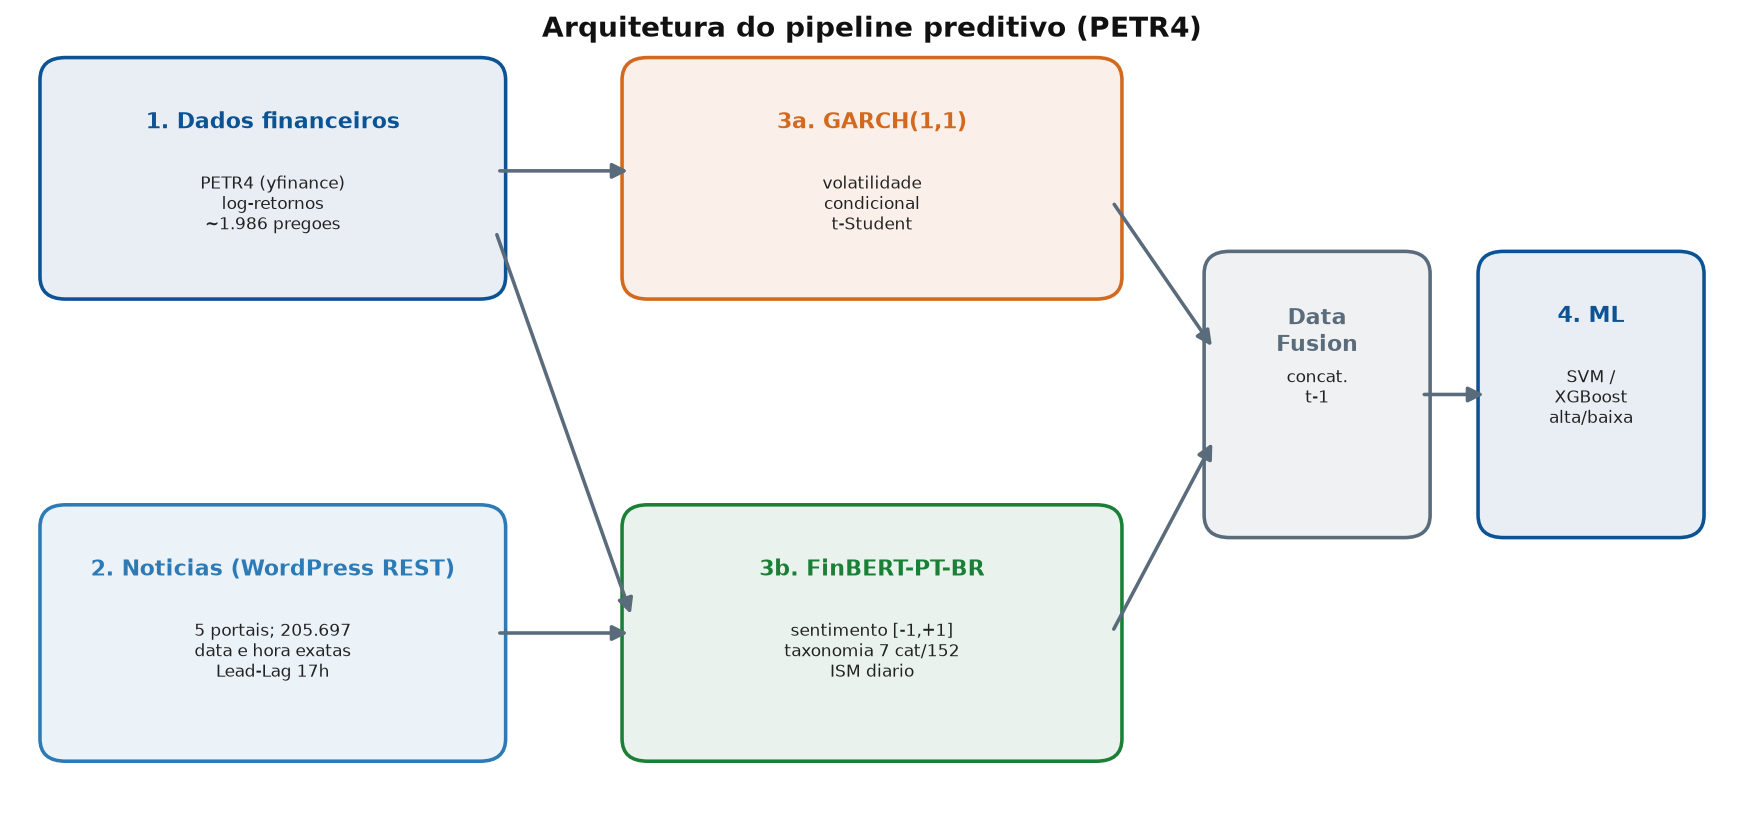
\includegraphics[width=0.95\textwidth]{figuras/arquitetura_pipeline_petr4.png}
\label{fig:arquitetura}
\vspace{0.2cm}
{\small Fonte: Elaborado pelo autor.}
\end{figure}

\section{Etapa 1: Dados Financeiros}

A variável dependente da pesquisa é o comportamento das ações preferenciais da Petrobras, negociadas sob o código PETR4. A escolha do ativo, já justificada no capítulo anterior, apoia-se na sua elevada liquidez e na sua dupla sensibilidade ao preço do petróleo e ao ambiente político doméstico. Coletaram-se as cotações diárias de fechamento, ajustadas para proventos, no período de 2018 a 2025, o que totaliza aproximadamente mil novecentos e oitenta e seis pregões.

A partir dos preços, calcula-se o log-retorno, métrica padrão em econometria financeira por aproximar a variação percentual e por favorecer a estacionariedade da série \cite{nizer_metodo_2011}. O log-retorno do dia $t$ é definido por
\begin{equation}
R_t = \ln\left(\frac{P_t}{P_{t-1}}\right),
\end{equation}
em que $P_t$ é o preço de fechamento no dia $t$ e $P_{t-1}$ o preço no pregão anterior. A variável-alvo da tarefa de direção é binária e deriva diretamente do sinal do log-retorno:
\begin{equation}
\text{Alvo}_t =
\begin{cases}
1 & \text{se } R_t > 0 \quad (\text{alta}),\\
0 & \text{se } R_t \le 0 \quad (\text{baixa}).
\end{cases}
\end{equation}
Não existe uma classe neutra na previsão direcional. O caso de retorno exatamente nulo, raríssimo em dados diários, é convencionado como baixa. Essa formulação binária é a mesma adotada pela literatura de previsão direcional, o que facilita a comparação com trabalhos anteriores \cite{ballings_evaluating_2015}.

\section{Etapa 2: Coleta de Notícias com Marcação Temporal}

Esta etapa corrige a falha mais grave apontada na qualificação. Na versão anterior, a impossibilidade de capturar o horário de publicação levou a uma imputação estocástica das datas, na qual as notícias foram distribuídas de forma aleatória pelos dias úteis. Como a banca observou com razão, esse procedimento desacopla a notícia da reação do mercado e invalida qualquer teste causal ou preditivo. A correção dessa falha é o eixo metodológico da presente versão.

A solução adotada é a coleta direta por meio da interface de programação dos portais de notícias. Muitos veículos de economia brasileiros operam sobre a plataforma WordPress, que expõe uma API no padrão REST, acessível pelo \textit{endpoint} \texttt{/wp-json/wp/v2/posts}. Essa interface retorna, para cada notícia, além do título e do resumo, dois campos temporais essenciais: o campo \texttt{date}, com a data e a hora de publicação no horário de Brasília, e o campo \texttt{date\_gmt}, com o mesmo instante em tempo universal coordenado. A disponibilidade desses campos garante a marcação temporal precisa que o método exige. Foram utilizados cinco portais, a saber, InfoMoney, Exame, MoneyTimes, Petronotícias e Poder360. O uso de múltiplas fontes atende a outra crítica da banca, pois mitiga o viés associado ao uso de um único veículo, que na versão anterior era o \textit{Valor Econômico}.

De posse da hora exata, aplica-se o alinhamento conhecido como \textit{Lead-Lag}. A regra é simples e tem fundamento econômico: notícias publicadas após o fechamento do pregão, fixado às dezessete horas no horário de Brasília, não podem influenciar o preço daquele mesmo dia, e por isso são atribuídas ao pregão do dia útil seguinte. Esse cuidado evita o vazamento de informação futura, que ocorreria se uma notícia da noite fosse associada ao fechamento já consumado. A relevância dessa precaução havia sido antecipada por \citeonline{gros-klusmann_when_2011} em seu estudo de reações intradiárias.

Cabe um registro sobre os aspectos éticos e legais da coleta. As notícias foram obtidas exclusivamente por interfaces públicas oferecidas pelos próprios portais, sem contornar mecanismos de autenticação, e armazenam-se apenas o título, o resumo e os metadados necessários à pesquisa, sem reprodução integral do conteúdo protegido. O uso é estritamente acadêmico e não comercial.

\subsection{Taxonomia Temática Supervisionada}

A versão de qualificação empregava a modelagem de tópicos por \textit{Latent Dirichlet Allocation}, escolha que a banca criticou em duas frentes. A primeira é conceitual: por se basear na contagem de palavras, o LDA representa um retrocesso em relação à semântica contextual do BERT, configurando um contrassenso dentro do mesmo \textit{pipeline}. A segunda é de validação: por ser não supervisionado, o LDA produz agrupamentos cuja interpretação depende de julgamento subjetivo, sem um critério objetivo de avaliação.

Em resposta, esta versão remove o LDA e adota uma taxonomia supervisionada, construída a partir da literatura econômica sobre os determinantes do preço da PETR4. A taxonomia organiza o vocabulário em sete categorias temáticas: empresa e Petrobras, mercado de petróleo, geopolítica, infraestrutura, sanções e navegação, governança, e macroeconomia e energia. Cada categoria reúne um conjunto de termos característicos, somando cento e cinquenta e dois termos no total. Uma notícia é atribuída a uma categoria quando contém termos a ela associados. A lista completa dos termos por categoria consta no Apêndice.

Essa abordagem traz três vantagens sobre o LDA. Primeiro, os grupos são interpretáveis e auditáveis, pois cada categoria corresponde a um conceito econômico definido a priori. Segundo, a categorização permite a análise de ablação, em que se mede a contribuição de cada vetor temático para a previsão, conforme se reporta no Capítulo~\ref{chap:resultados}. Terceiro, e mais importante para a coerência do estudo, a taxonomia viabiliza a distinção entre eventos da empresa e eventos do mercado de petróleo, que é a chave para tratar a assimetria descrita por \citeonline{kilian_not_2009} e discutida no capítulo anterior. Uma notícia sobre o fechamento de uma rota de transporte de petróleo, por exemplo, é classificada na categoria de mercado, o que sinaliza ao sistema que o seu efeito sobre a produtora pode ser oposto ao seu efeito sobre o índice geral.

\subsection{Tratamento e pré-processamento do corpus textual}

O texto bruto coletado dos portais não está pronto para a análise e exige uma sequência de tratamentos, registrada aqui em detalhe por ser parte essencial do método. A primeira operação é a engenharia de atributos textuais por concatenação. Para cada notícia, os campos de título e de resumo são unidos em uma única sentença, o que fornece ao modelo de linguagem um contexto mais rico do que o título isolado ofereceria. Essa decisão alinha-se à constatação de \citeonline{hagenau_automated_2013} de que atributos sensíveis ao contexto da sentença elevam a acurácia, e mantém-se coerente com a hipótese de eficiência informacional, segundo a qual o título e o primeiro parágrafo concentram a informação mais saliente de uma notícia.

A segunda operação é a remoção de duplicatas. Como cinco portais são consultados e uma mesma notícia de agência pode ser republicada, calcula-se um resumo criptográfico do título de cada registro, e mantém-se apenas a primeira ocorrência de cada resumo. Esse procedimento evita que uma notícia repetida infle artificialmente o índice de sentimento de um pregão.

A terceira operação é uma limpeza leve de qualidade. Aqui foi tomada uma decisão metodológica importante, em contraste com uma filtragem agressiva. A literatura adverte que o volume bruto de publicações não se traduz integralmente em sinal preditivo \cite{nizer_metodo_2011}, o que poderia sugerir uma filtragem severa. Optou-se, porém, por uma limpeza leve, que remove apenas os registros degenerados, como títulos vazios, com menos de quinze caracteres ou compostos somente de marcadores de navegação. Da base bruta de duzentas e cinco mil setecentas e dezesseis notícias, foram removidos apenas dezenove registros, e preservaram-se duzentas e cinco mil seiscentas e noventa e sete. A razão para a limpeza leve é dupla. Primeiro, preserva a integralidade do corpus para a análise de ablação, que depende de notícias de todas as categorias, inclusive das exógenas de geopolítica e macroeconomia. Segundo, evita a subjetividade de um critério de relevância que poderia, ele próprio, introduzir viés ao descartar notícias com base em uma definição prévia de importância. A base bruta original é mantida intacta, e todas as bases derivadas são geradas a partir dela por roteiros reproduzíveis, sem edição manual.

\section{Etapa 3a: Extração de Sentimento via FinBERT-PT-BR}

A extração do sentimento emprega o FinBERT-PT-BR \cite{santos_finbert_2023}, o modelo BERTimbau ajustado ao domínio financeiro. Convém esclarecer com precisão o procedimento de extração do escore, uma vez que a banca observou, corretamente, que o BERT é um codificador e não um classificador por construção. O processo se dá em três passos.

\begin{enumerate}
    \item \textbf{Codificação e cabeçalho de classificação.} O texto da notícia, formado pela concatenação do título com o resumo, é processado pelo codificador, que produz uma representação vetorial contextual. A essa representação acopla-se um cabeçalho de classificação de três classes, positivo, negativo e neutro, que foi ajustado durante o \textit{fine-tuning} financeiro do modelo.
    \item \textbf{Normalização por \textit{softmax}.} Os valores brutos produzidos pelo cabeçalho, chamados \textit{logits}, são convertidos em probabilidades pela função \textit{softmax}. O resultado é o rótulo vencedor e a sua confiança $c \in [0,1]$, que mede o grau de certeza do modelo naquela classificação.
    \item \textbf{Construção do índice contínuo.} Atribui-se à polaridade um valor $p \in \{+1, 0, -1\}$ conforme o rótulo seja positivo, neutro ou negativo. O índice de sentimento da notícia é então o produto $s = p \times c$, que assume valores no intervalo $[-1, +1]$.
\end{enumerate}

A banca indagou se o sentimento contínuo comporta intervalos de interpretação. A resposta é afirmativa. Embora a aplicação preditiva utilize o valor contínuo $s$, para fins de leitura qualitativa consideram-se três faixas: a faixa negativa, em $[-1, -0{,}05)$; a faixa neutra, em $[-0{,}05, +0{,}05]$; e a faixa positiva, em $(+0{,}05, +1]$. A faixa neutra estreita em torno de zero evita classificar como portadora de sinal uma notícia cuja polaridade é, na prática, indefinida.

\subsection{Construção do Índice de Sentimento da Mídia}

O Índice de Sentimento da Mídia, ou ISM, de um pregão é a média aritmética dos índices $s$ de todas as notícias a ele atribuídas após o alinhamento \textit{Lead-Lag}. Formalmente, para um pregão $t$ ao qual foram atribuídas $n_t$ notícias com índices $s_{1}, \dots, s_{n_t}$, define-se
\begin{equation}
\text{ISM}_t = \frac{1}{n_t} \sum_{i=1}^{n_t} s_{i}.
\end{equation}
Quando um mesmo dia reúne notícias positivas e negativas, elas se compensam na média, e o que resta é o saldo líquido de sentimento daquele pregão. Uma propriedade desejável dessa construção é que ela preserva a intensidade: uma notícia classificada com alta confiança pesa mais, em módulo, do que uma notícia quase neutra. O Capítulo~\ref{chap:resultados} investiga ainda uma variante ponderada pela confiança, que atribui peso proporcional à certeza de cada classificação, e compara o seu desempenho ao da média simples.

\subsection{Validação humana do modelo}

Em atenção à recomendação da banca de validar o sentimento automático por meio de rotulagem manual, construiu-se um conjunto-ouro. Trata-se de uma amostra de trezentas notícias, selecionadas de forma estratificada por classe de sentimento e por ano, de modo a cobrir todo o período e a garantir representação da classe minoritária. Essas notícias são rotuladas manualmente, sem que o rótulo do modelo seja exibido ao anotador, o que evita o viés de ancoragem. Contra esse padrão de referência, medem-se a acurácia do FinBERT-PT-BR e o coeficiente \textit{kappa} de Cohen \cite{cohen_coefficient_1960}, que quantifica a concordância entre o modelo e o anotador humano para além do que se esperaria do acaso. A construção e a avaliação desse conjunto compõem a etapa final de validação rumo à defesa.

\section{Etapa 3b: Modelagem Econométrica do Risco}

Para que a volatilidade atue como variável de controle e como objeto de estudo, a variância condicional da PETR4 é estimada por um modelo GARCH(1,1) \cite{bollerslev_generalized_1986}, com distribuição \textit{t}-Student dos resíduos, adequada às caudas pesadas das séries financeiras. O modelo é definido por
\begin{equation}
\sigma_t^2 = \omega + \alpha\,\epsilon_{t-1}^2 + \beta\,\sigma_{t-1}^2,
\end{equation}
em que $\sigma_t^2$ é a variância condicional prevista para o dia $t$; $\omega$ é a constante associada à variância de longo prazo; o termo $\alpha\,\epsilon_{t-1}^2$ captura o impacto dos choques recentes, isto é, das surpresas informacionais do dia anterior; e o termo $\beta\,\sigma_{t-1}^2$ representa a inércia da volatilidade, ou seja, a sua tendência a persistir. A soma $\alpha + \beta$ mede a persistência total da volatilidade.

A escolha do GARCH(1,1), e não de uma especificação alternativa, responde a uma pergunta direta da banca e apoia-se em três argumentos. O primeiro é a parcimônia. A especificação com uma defasagem de cada termo é a mais simples capaz de reproduzir o agrupamento de volatilidade, e a literatura mostra que raramente é superada por ordens superiores na previsão de séries diárias de ações. O segundo é a robustez empírica em mercados emergentes, nos quais o GARCH(1,1) é o modelo de referência consolidado, inclusive em estudos do mercado brasileiro \cite{silva_o_2018}. O terceiro é a comparabilidade, pois a adoção da mesma especificação empregada na literatura correlata permite confrontar os resultados de forma direta. Especificações assimétricas, como o EGARCH, que capturam o efeito de alavancagem segundo o qual choques negativos elevam mais a volatilidade do que choques positivos, são reconhecidas como extensão pertinente e registradas entre os trabalhos futuros. A adequação do ajuste é verificada pela análise dos resíduos padronizados, reportada no Capítulo~\ref{chap:resultados}.

\section{Etapa 4: Fusão de Dados e Classificadores}

A pergunta da banca sobre se a fusão de dados seria uma mera concatenação de atributos merece uma resposta formal. A fusão de dados, neste trabalho, é a construção de uma matriz na qual cada linha corresponde a um pregão e reúne atributos de natureza heterogênea, todos defasados em um dia. Para prever a direção do pregão $t$, o vetor de atributos é
\begin{equation}
\mathbf{x}_t = \left[\, R_{t-1},\ \sigma_{t-1},\ \text{ISM}_{t-1} \,\right],
\end{equation}
em que $R_{t-1}$ é o log-retorno do dia anterior, $\sigma_{t-1}$ é a volatilidade condicional estimada pelo GARCH para o dia anterior, e $\text{ISM}_{t-1}$ é o índice de sentimento do dia anterior. A defasagem uniforme em $t-1$ é o que garante o respeito ao pressuposto de causalidade temporal, pois assegura que a previsão de hoje use apenas informação de ontem. A justificativa teórica para combinar essas fontes complementares, a quantitativa e a textual, é a fundamentação de fusão de dados de \citeonline{barak_fusion_2017}, reforçada pelos resultados de \citeonline{li_incorporating_2020}.

A tarefa de classificação binária, que atribui o rótulo um para alta e zero para baixa, é resolvida por dois algoritmos não lineares. O primeiro é a máquina de vetores de suporte, ou SVM, que busca a fronteira de separação de margem máxima entre as classes e, por meio de funções de \textit{kernel}, é capaz de modelar relações não lineares em espaços de baixa dimensão. O segundo é o \textit{Extreme Gradient Boosting}, ou XGBoost \cite{chen_xgboost_2016}, um método de \textit{boosting} que combina muitas árvores de decisão rasas, cada uma corrigindo os erros das anteriores, e que se consolidou como estado da arte para dados tabulares por sua robustez ao sobreajuste e por fornecer medidas de importância dos atributos, úteis na análise de ablação. A escolha desses dois algoritmos é amparada pela avaliação de classificadores de \citeonline{ballings_evaluating_2015} e pela eficácia do XGBoost demonstrada por \citeonline{nobre_combining_2019}. A decisão final do classificador opera por probabilidade: o modelo estima a probabilidade de alta $\hat{p} \in [0,1]$, e decide-se pela alta quando $\hat{p} \ge 0{,}5$, e pela baixa em caso contrário.

\subsection{Protocolo de validação e justificativa das métricas}

A avaliação de modelos sobre séries temporais exige cuidado especial para evitar o vazamento de informação. A validação cruzada tradicional, que embaralha as observações, permitiria ao modelo treinar com dados do futuro para prever o passado, um erro grave em finanças. Para evitá-lo, adota-se a divisão estritamente cronológica em três partes, na proporção de sessenta, quinze e vinte e cinco por cento, destinadas respectivamente ao treino, à validação e ao teste. O conjunto de treino ajusta os parâmetros dos modelos. O conjunto de validação serve à seleção de hiperparâmetros e de atributos. O conjunto de teste, formado pelos pregões mais recentes, é consultado uma única vez, ao final, e fornece a estimativa não enviesada do desempenho fora da amostra.

As métricas de avaliação foram escolhidas de forma deliberada, e cada uma cumpre um papel. A acurácia mede a proporção de acertos e é diretamente comparável ao patamar de cinquenta por cento que a Hipótese de Mercados Eficientes estabelece como referência. A precisão e o F1-Score são relevantes porque as classes de alta e baixa podem ser desbalanceadas, e essas métricas penalizam modelos que acertam uma classe à custa da outra. A área sob a curva ROC, ou AUC, mede a capacidade do modelo de ordenar corretamente os pregões por probabilidade de alta, independentemente do limiar de decisão escolhido. Além dessas métricas, reportam-se duas linhas de base, a previsão pela classe majoritária e o modelo baseado apenas em preços, e dois testes de significância estatística, o teste binomial e o teste de McNemar, que aferem, respectivamente, se o modelo supera o acaso e se a adição do sentimento produz ganho estatisticamente distinguível.

\subsection{Configuração concreta da modelagem}

Para fins de reprodutibilidade, registram-se os parâmetros efetivos da modelagem. A divisão cronológica aplicada sobre os aproximadamente mil novecentos e oitenta e seis pregões resultou em mil cento e noventa e um pregões de treino, que cobrem de janeiro de 2018 a outubro de 2022, duzentos e noventa e oito pregões de validação, de outubro de 2022 a janeiro de 2024, e quatrocentos e noventa e sete pregões de teste, de janeiro de 2024 a dezembro de 2025. Convém notar, desde já, que a proporção de pregões de alta difere entre a validação e o teste, fato que se revelará determinante na interpretação do estudo de refinamento, no Capítulo~\ref{chap:resultados}.

A configuração de referência do XGBoost emprega trezentas árvores, profundidade máxima de três níveis, taxa de aprendizado de zero vírgula zero cinco e subamostragem de noventa por cento das observações e dos atributos a cada árvore, valores escolhidos por equilibrarem capacidade e regularização em uma matriz de poucos atributos. A máquina de vetores de suporte utiliza núcleo de base radial, precedida de uma padronização dos atributos ajustada estritamente sobre a janela de treino, de modo a impedir qualquer contaminação do teste. O estudo de refinamento, reportado adiante, parte dessa configuração e investiga, de forma sistemática, o efeito de alterá-la.

\section{Exemplo Didático}

Para tornar o método concreto, acompanha-se uma notícia hipotética por todo o \textit{pipeline}. Suponha-se que, às dezoito horas de uma terça-feira, um portal publique a manchete: \textit{Guerra no Oriente Médio fecha o Estreito de Ormuz e ameaça o transporte de petróleo}.

\begin{enumerate}
    \item \textbf{Coleta.} A notícia é capturada pela API com a sua data e hora exatas, dezoito horas.
    \item \textbf{Alinhamento.} Como dezoito horas é posterior ao fechamento das dezessete horas, a notícia é atribuída ao pregão da quarta-feira, e não ao da terça já encerrado.
    \item \textbf{Categorização.} Os termos Estreito de Ormuz e petróleo classificam a notícia nas categorias de geopolítica e mercado de petróleo.
    \item \textbf{Sentimento.} O FinBERT-PT-BR identifica tom negativo, pela presença de guerra e ameaça, e atribui um escore, por exemplo, $s = -0{,}7$.
    \item \textbf{Agregação.} Esse valor entra na média que forma o ISM da quarta-feira, junto com as demais notícias do período.
    \item \textbf{Fusão e leitura econômica.} O ISM, defasado, compõe o vetor de atributos ao lado do retorno e da volatilidade de ontem. Embora o tom seja negativo, a categoria de mercado sinaliza um choque de oferta, que tende a elevar o preço do petróleo e pode favorecer a produtora. O classificador pondera esse sinal junto aos demais atributos para estimar a probabilidade de alta.
\end{enumerate}

Esse percurso evidencia como o método distingue uma notícia negativa para o mercado de uma negativa para a empresa, questão que a banca considerou central.

\section{Reprodutibilidade}

Todo o \textit{pipeline} foi implementado em linguagem Python e executado localmente. A análise de sentimento utiliza as bibliotecas \textit{Transformers} e PyTorch para a inferência do FinBERT-PT-BR. A modelagem econométrica emprega a biblioteca \textit{arch} para o GARCH. Os classificadores utilizam as bibliotecas \textit{scikit-learn}, para o SVM, e \textit{xgboost}, para o XGBoost. As sementes dos geradores de números aleatórios foram fixadas, e as versões das bibliotecas foram registradas, de modo a permitir a reprodução dos resultados. Os detalhes do ambiente computacional constam no Apêndice.
